\subsection{Bestimmung der Strömungsgeschwingigkeiten}

Die eingehende Frequenz liegt bei
\begin{align*}
  \nu_{\text{0}}=\SI{2}{MHz}.
\end{align*}
Der Dopplerwinkel $\alpha$ wird mit Gleichung \eqref{eqn:alpha} errechnet.
Die jeweiligen Dopplerwinkel sind mit ihren Prismenwinkeln $\theta$ in Tabelle \ref{tab:alpha} notiert.
\begin{table}[h!]
  \centering
  \caption{Prismenwinkel $\theta$ und die sich ergebenden Dopplerwinkel $\alpha$}
  \label{tab:alpha}
  \begin{tabular}{c c}
    \toprule
      $\theta/°$  &  $\alpha/°$     \\
      \midrule
    15  &   80,06 \\
    30  &   70,53 \\
    60  &   54,74 \\
    \bottomrule
  \end{tabular}
\end{table}

%\end{landscape}
%\end{document}

%\begin{align}
%  \frac{\Delta \nu}{\cos{(\alpha)}}= \frac{2 \nu_{\text{0}}}{c}\cdot v\\
%  \frac{c \Delta \nu}{2 \nu_{\text{0}}\cos{(\alpha)}}= v\\
%\end{align}
Die Flussgeschwindigkeit berechnet sich über Gleichung \eqref{eqn:v}.
Als Schallgeschwindigkeit wird
\begin{align*}
  c_L=\SI{1800}{\frac{m}{s}}
\end{align*}
verwendet.
Die Messwerte zu den Flussgeschwindigkeiten sind in Tabelle \ref{tab:v} aufgetragen.
%\begin{landscape}


\begin{table}[h!]
  \centering
  \caption{Messergebnisse zur Strömungsgeschwindigkeit $v$}
  \label{tab:v}
  \begin{tabular}{c c c c c c c c c c c c c c c c c c c c c c c}
    \toprule
          -   &  \multicolumn{3}{c}{$r=\SI{0.0035}{m}$} & \multicolumn{3}{c}{$r=\SI{0.005}{m}$} & \multicolumn{3}{c}{$r=\SI{0.008}{m}$}\\
      \midrule
    $\theta/°$ & $ \vert \Delta \nu \vert$ /Hz & $\frac{\vert \Delta \nu \vert}{\cos{(\alpha)}}$/Hz & $v/\frac{m}{s}$ &    $\vert \Delta \nu \vert$/Hz & $\frac{\vert \Delta \nu \vert} {\cos{(\alpha)}}$/Hz & $v/\frac{m}{s}$ & $\vert \Delta \nu \vert$/Hz & $\frac{\vert \Delta \nu \vert}{\cos{(\alpha)}}$/Hz &$v/\frac{m}{s}$\\
      \midrule
      \multicolumn{10}{c}{$\dot{V}=\SI{2,3}{l/min}$}\\
      \midrule
    15	&     195   & 1129 &  0,508  &     122  & 706  &  0,318  &      61   & 353 &  0,159 \\
    30	&     366   & 1098 &  0,494  &     183  & 549  &  0,247  &      98   & 294 &  0,132 \\
    60	&     671   & 1162 &  0,523  &     330  & 571  &  0,257  &     134   & 232 &  0,105 \\
      \midrule
      \multicolumn{10}{c}{$\dot{V}=\SI{3,0}{l/min}$}\\
      \midrule
    15	&     305   & 1766 &  0,795  &     159  & 921  &  0,415  &      85   & 492 &  0,222 \\
    30	&     562   & 1686 &  0,759  &     281  & 843  &  0,379  &     134   & 402 &  0,181 \\
    60	&     1050  & 1818 &  0,818  &     531  & 919  &  0,414  &     208   & 360 &  0,162 \\
      \midrule
      \multicolumn{10}{c}{$\dot{V}=\SI{3,5}{l/min}$}\\
      \midrule
    15	&     354   & 2050 &  0,923  &     208  & 1204  &  0,542  &    98    & 567 &  0,256 \\
    30	&     787   & 2361 &  1,063  &     366  & 1098  &  0,494  &    171   & 513 &  0,231 \\
    60	&     1331  & 2305 &  1,038  &     690  & 1195  &  0,539  &    269   & 465 &  0,210 \\
      \midrule
      \multicolumn{10}{c}{$\dot{V}=\SI{4}{l/min}$}\\
      \midrule
    15	&     588   & 3406 &  1,533  &     244  & 1413  &  0,636  &    122   & 706 &  0,318 \\
    30	&     977   & 2931 &  1,319  &     488  & 1464  &  0,659  &    232   & 696 &  0,313 \\
    60	&     1758  & 3045 &  1,370  &     916  & 1586  &  0,714  &    342   & 592 &  0,267 \\
      \midrule
      \multicolumn{10}{c}{$\dot{V}=\SI{4,5}{l/min}$}\\
      \midrule
    15	&     586   & 3394 &  1,528  &     317  & 1836  &  0,826  &    159   & 921 &  0,415 \\
    30	&     1306  & 3918 &  1,763  &     586  & 1758  &  0,791  &    293   & 879 &  0,396 \\
    60	&     2124  & 3679 &  1,656  &     1221 & 2115  &  0,952  &    464   & 803 &  0,362 \\

    \bottomrule
  \end{tabular}
\end{table}

%\end{landscape}

Die Strömungsgeschwindigkeiten werden für die unterschiedlichen Prismenwinkel gegen $\frac{\Delta \nu}{\cos{\alpha}}$ in den Abbildungen \ref{fig:15}, \ref{fig:30} und \ref{fig:60} aufgetragen.
\begin{figure}[h!]
  \centering
  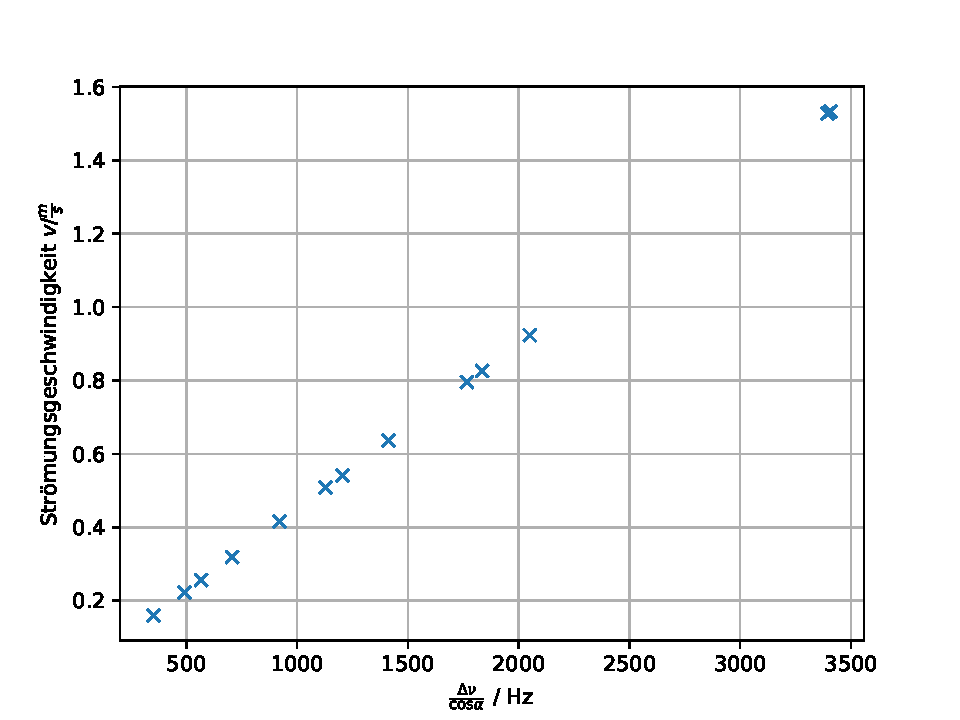
\includegraphics[width=\textwidth]{15geschw.pdf}
  \caption{$v$ gegen $\frac{\Delta \nu}{\cos{\alpha}}$ für den Winkel $\theta=\SI{15}{°}$}
  \label{fig:15}
\end{figure}
%
\begin{figure}[h!]
  \centering
  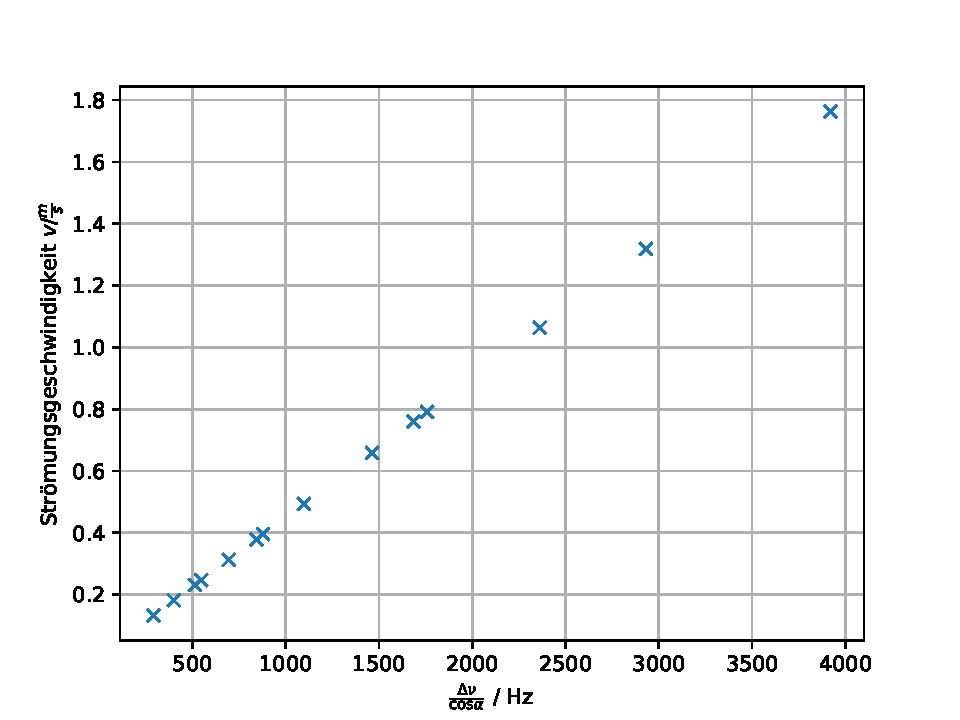
\includegraphics[width=\textwidth]{30geschw.pdf}
  \caption{$v$ gegen $\frac{\Delta \nu}{\cos{\alpha}}$ für den Winkel $\theta=\SI{30}{°}$}
  \label{fig:30}
\end{figure}
%
\begin{figure}[h!]
  \centering
  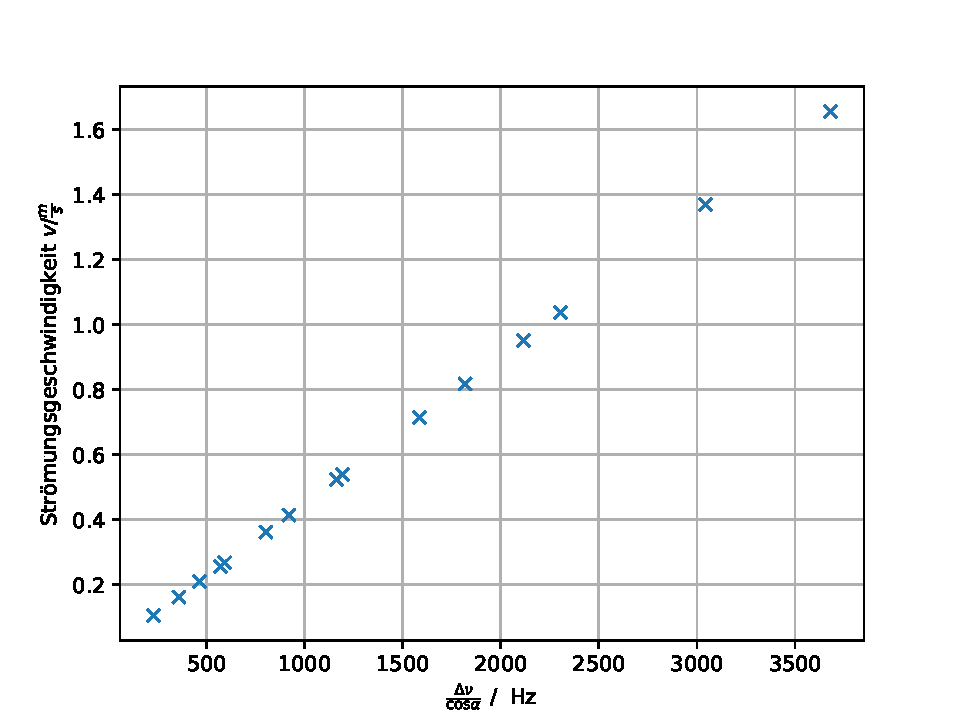
\includegraphics[width=\textwidth]{60geschw.pdf}
  \caption{$v$ gegen $\frac{\Delta \nu}{\cos{\alpha}}$ für den Winkel $\theta=\SI{60}{°}$}
  \label{fig:60}
\end{figure}

\FloatBarrier

\subsection{Bestimmung des Strömungsprofils}
Die Messung wird bei $x=\SI{12}{\mu s}$ gestartet, da mit der Umrechnung $\SI{4}{\mu s}= \SI{10e-3}{m}$ ersichtlich wird, dass eine Messung erst ab einer Tiefe von $l=\SI{30.7e-3}{m}=\SI{12.28}{\mu s}$ sinnvoll ist.
Erst nach der Länge $l$ tritt der Schall aus dem Prisma in die Dopplerflüssigkeit.
Die Messtiefe $x=\SI{12}{\mu s}$ entspricht dem Beginn des Rohrs mit $s=\SI{0}{mm}$
Die Messwerte zur Bestimmung des Strömungsprofils sind in Tabelle \ref{tab:profil} notiert.
\begin{table}[h!]
  \centering
  \caption{Messwerte zum Strömungsprofil. Messtiefe $x$ in $\mu s$ und $mm$, Frequenzverschiebung $\Delta \nu$, Flussgeschwindigkeit $v$, Steuintensität $I$}
  \label{tab:profil}
  \begin{tabular}{c c c c c c c c}
    \toprule
                &         & \multicolumn{3}{c}{$\dot{V}=\SI{4,8}{l/min}$} & \multicolumn{3}{c}{$\dot{V}=\SI{3,4}{l/min}$} \\
      $x/\mu s$ & $s/mm$  &  $\Delta \nu / Hz$ & $v/\frac{m}{s}$ & $I$ &  $\Delta \nu / Hz$ & $v/\frac{m}{s}$ & $I$    \\
      \midrule
      12,0      & 0,000   &   195  &  0,508  &  10,8   & 146   &   0,381  &  10,0 \\
      12,5      & 0,750  &   232  &  0,605  &   9,2   & 183   &   0,477  &   8,3 \\
      13,0      & 1,500  &   330  &  0,860  &   5,1   & 220   &   0,574  &   6,6 \\
      13,5      & 2,250  &   439  &  1,144  &   4,5   & 281   &   0,733  &   3,2 \\
      14,0      & 3,000  &   537  &  1,400  &   3,9   & 330   &   0,860  &   4,0 \\
      14,5      & 3,750  &   562  &  1,465  &   2,3   & 354   &   0,922  &   3,5 \\
      15,0      & 4,500  &   586  &  1,528  &   2,5   & 366   &   0,954  &   3,2 \\
      15,5      & 5,250  &   549  &  1,431  &   3,0   & 342   &   0,892  &   3,4 \\
      16,0      & 6,000  &   452  &  1,178  &   2,9   & 281   &   0,733  &   4,0 \\
      16,5      & 6,750  &   317  &  0,826  &   5,5   & 208   &   0,542  &  10,0 \\
      17,0      & 7,500  &   220  &  0,574  &   9,2   & 171   &   0,446  &   9,0 \\
      17,5      & 8,250  &   208  &  0,542  &  10,2   & 146   &   0,381  &  14,2 \\
      18,0      & 9,000  &   269  &  0,701  &  13,4   & 208   &   0,542  &  12,7 \\
      18,5      & 9,750  &   317  &  0,826  &   9,8   & 232   &   0,605  &   9,7 \\
      19,0      & 10,50  &   342  &  0,892  &  10,0   & 208   &   0,542  &   7,8 \\
      19,5      & 11,25  &   360  &  0,939  &   7,3   & 195   &   0,508  &   6,6 \\

    \bottomrule
  \end{tabular}
\end{table}

%\end{landscape}
%\end{document}

Die Messwerte sind für die jeweiligen Volumenströme $\dot{V}$ in den Abbildungen \ref{fig:40i}, \ref{fig:40v}, \ref{fig:65i} und \ref{fig:65v} aufgetragen.
\begin{figure}[h!]
  \centering
  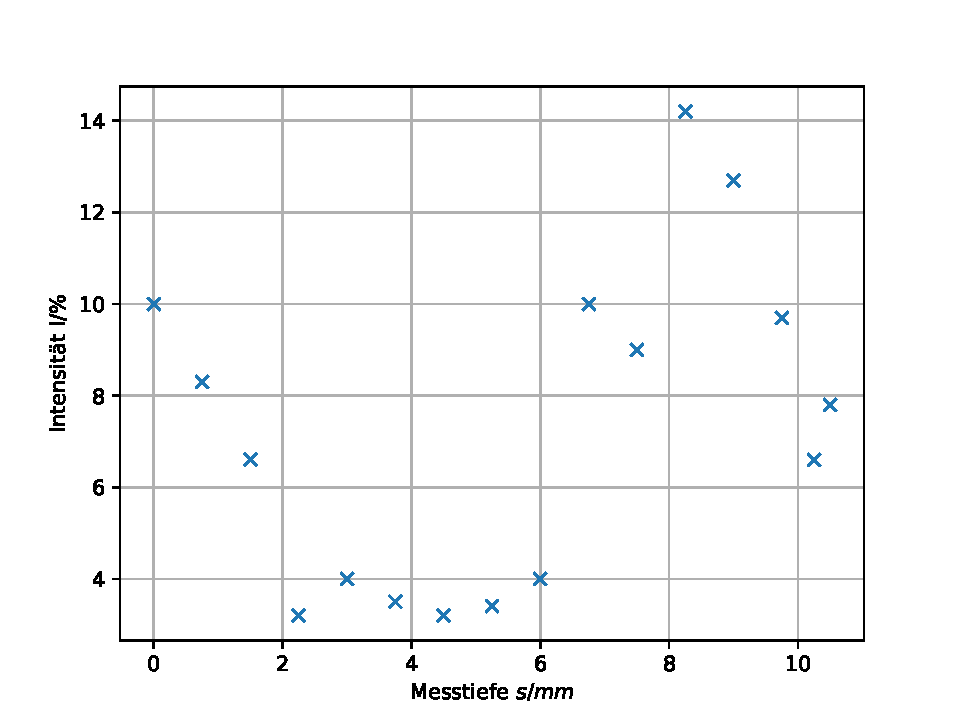
\includegraphics[width=\textwidth]{40prozi.pdf}
  \caption{Streuintensität $I$ gegen die Messtiefe $s$ für $\dot{V}=\SI{3,4}{l/min}$}
  \label{fig:40i}
\end{figure}
%
\begin{figure}[h!]
  \centering
  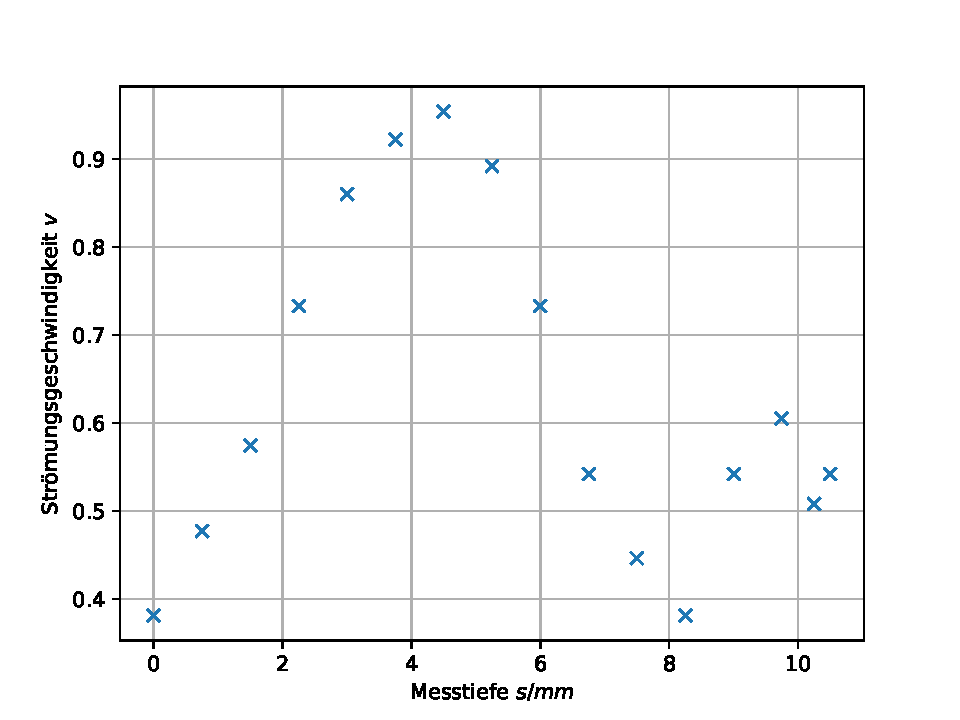
\includegraphics[width=\textwidth]{40prozv.pdf}
  \caption{Flussgeschwindigkeit $v$ gegen die Messtiefe $s$ für $\dot{V}=\SI{3,4}{l/min}$}
  \label{fig:40v}
\end{figure}
%
\begin{figure}[h!]
  \centering
  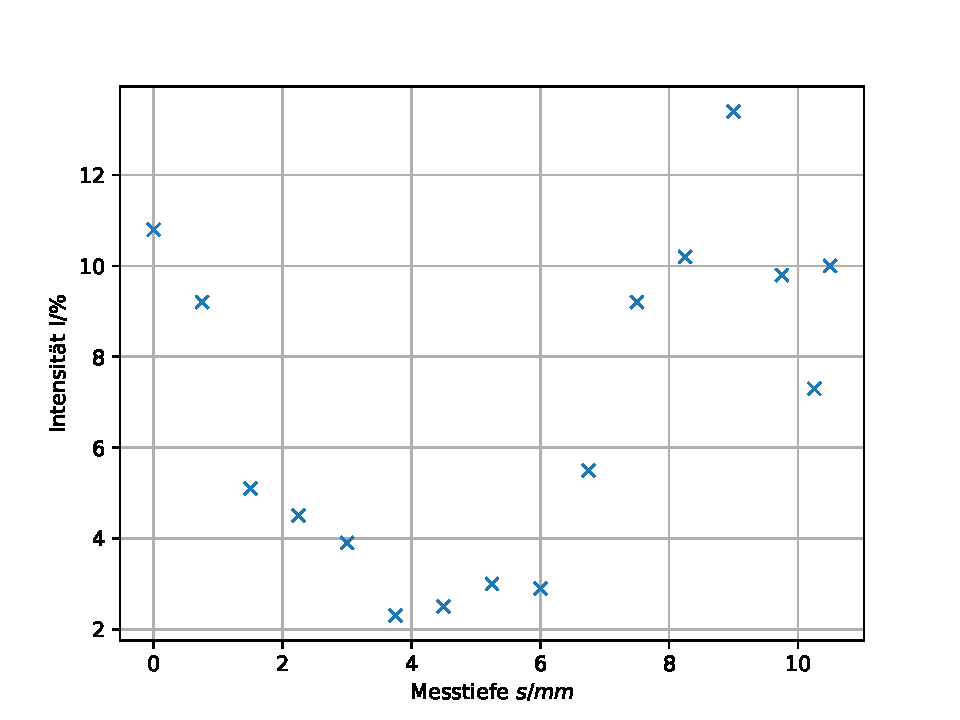
\includegraphics[width=\textwidth]{65prozi.pdf}
  \caption{Streuintensität $I$ gegen die Messtiefe $s$ für $\dot{V}=\SI{4,8}{l/min}$}
  \label{fig:65i}
\end{figure}
%
\begin{figure}[h!]
  \centering
  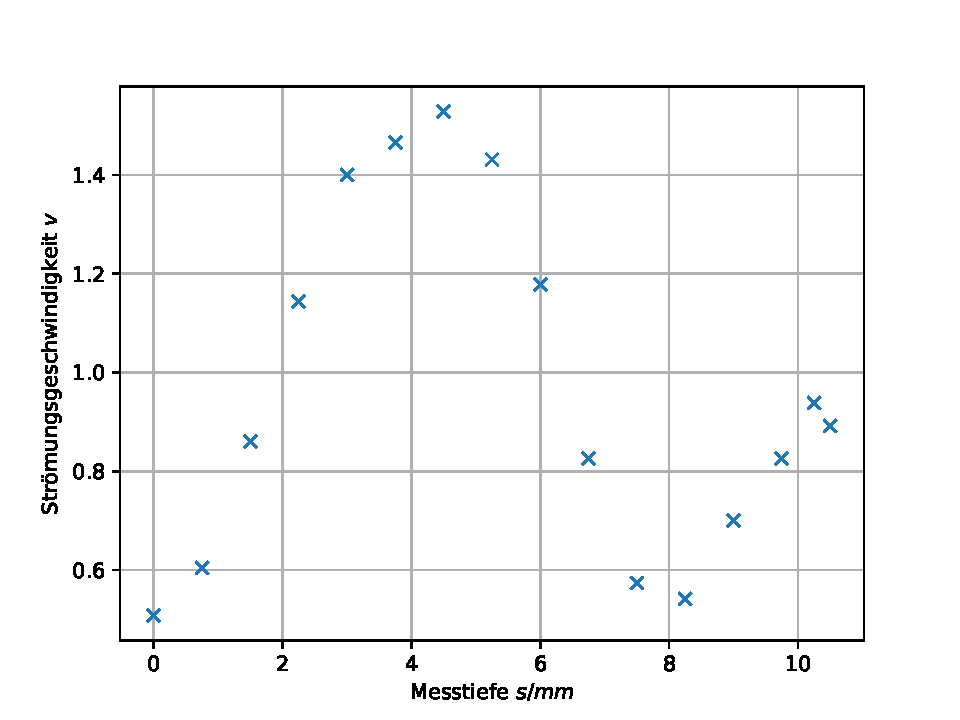
\includegraphics[width=\textwidth]{65prozv.pdf}
  \caption{Flussgeschwindigkeit $v$ gegen die Messtiefe $s$ für $\dot{V}=\SI{4,8}{l/min}$}
  \label{fig:65v}
\end{figure}
Zur Bestimmung eines Referenzwertes werden die ersten zwölf Messwerte gemittelt um die mittlere Flussgeschwindigkeit zu errechnen.
Ein Mittelwert berechnet sich durch die Anzahl der Messwerte $N$
\begin{align*}
  \bar{x}=\frac{1}{N} \left( \sum^{N}_{n=1} x_n \right).
\end{align*}
Es ergeben sich folgende Mittelwerte:
\begin{align*}
  \bar{v}_{3,4 l/min}= & \SI{0.658}{\frac{m}{s}} \\
  \bar{v}_{4,8 l/min}= & \SI{1.005}{\frac{m}{s}} \\
\end{align*}
Als theoretische Vergleichswerte der Flussgeschwindigkeit werden mit dem Kontinuitätsgesetz der Hydrodynamik
\begin{align}
  \dot{V}=A v \Leftrightarrow v= \frac{\dot{V}}{A}
  \label{eqn:konti}
\end{align}
berechnet.
Die theoretischen Flussgeschwindigkeiten für den Rohrradius $r=\SI{5e-3}{m}$ und beiden Volumenströme berechnen sich zu:
\begin{align*}
  v_{\text{theo, 3,4 l/min}}=& \SI{0.722}{\frac{m}{s}} \\
  v_{\text{theo, 4,8 l/min}}=& \SI{1.019}{\frac{m}{s}} \\
\end{align*}


\FloatBarrier
